\documentclass[a4paper, titlepage]{article}
\usepackage[round, sort, numbers]{natbib}
\usepackage[utf8]{inputenc}
\usepackage{amsfonts, amsmath, amssymb, amsthm}
\usepackage{color}
\usepackage{listings}
\usepackage{marvosym}
\usepackage{mathtools}
\usepackage{paralist}
\usepackage{parskip}
\usepackage{subfig}
\usepackage{tikz}
\usepackage{titlesec}

\numberwithin{figure}{section}
\numberwithin{table}{section}

\usetikzlibrary{arrows, automata, backgrounds, petri, positioning}
\tikzstyle{place}=[circle, draw=blue!50, fill=blue!20, thick]
\tikzstyle{transition}=[rectangle, draw=black!50, fill=black!20, thick]

% define new commands for sets and tuple
\newcommand{\setof}[1]{\ensuremath{\left \{ #1 \right \}}}
\newcommand{\tuple}[1]{\ensuremath{\left \langle #1 \right \rangle }}
\newcommand{\card}[1]{\ensuremath{\left \vert #1 \right \vert }}

\makeatletter
\newcommand\objective[1]{\def\@objective{#1}}
\newcommand{\makecustomtitle}{%
	\begin{center}
		\huge\@title \\
		[1ex]\small Aurélien Coet, Dimitri Racordon
	\end{center}
	\@objective
}
\makeatother

\begin{document}

  \title{Outils formels de Modélisation \\ 3\textsuperscript{ème} séance d'exercices}
  \author{Aurélien Coet, Dimitri Racordon}
	\objective{
		Dans cette séance d'exercices, nous allons étudier et manipuler le comportement de réseaux de Petri en utilisant la simulation.
	}

	\makecustomtitle

  \section{Simulations [\Keyboard] ($\bigstar\bigstar$)}
    Représentez le réseau de Petri de la figure \ref{fig:bezout} en F\#,
    puis répondez aux questions suivantes:

    \begin{enumerate}
			\item La transition $t_2$ est-elle tirable?
			\item Donnez un marquage possible du réseau après 100 tirs de transitions.
            \item Le nombre de jetons dans le réseau est-il borné ?
		\end{enumerate}

    \begin{figure}[ht]
      \centering
        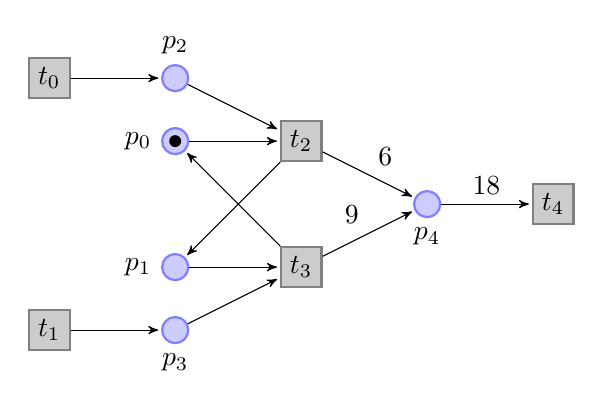
\begin{tikzpicture}[node distance=16mm, >=stealth', bend angle=45, auto]
          \node[place] (p4) [label=below:$p_4$] {};
          \node[place,tokens=1] (p0) [left of=p4,xshift=-16mm,yshift=8mm,label=left:$p_0$] {};
          \node[place] (p1) [left of=p4,xshift=-16mm,yshift=-8mm,label=left:$p_1$] {};
          \node[place] (p2) [above of=p0,yshift=-8mm,label=above:$p_2$] {};
          \node[place] (p3) [below of=p1,yshift=8mm,label=below:$p_3$] {};

          \node [transition] (t0) [left of=p2] {$t_0$}
                edge [post] (p2);
          \node [transition] (t1) [left of=p3] {$t_1$}
                edge [post] (p3);
          \node [transition] (t2) [right of=p0] {$t_2$}
                edge [pre] (p0)
                edge [pre] (p2)
                edge [post] node {6} (p4)
                edge [post] (p1);
          \node [transition] (t3) [right of=p1] {$t_3$}
                edge [pre] (p1)
                edge [pre] (p3)
                edge [post] node {9} (p4)
                edge [post] (p0);
          \node [transition] (t4) [right of=p4] {$t_4$}
                edge [pre] node[swap] {18} (p4);
        \end{tikzpicture}
      \caption{Réseau exposant des propriétés algébriques intéressantes}
      \label{fig:bezout}
    \end{figure}

  \section{Complémentaire mon cher [\Keyboard] ($\bigstar\bigstar$)}
  Il est parfois désirable de limiter le nombre de jetons qui peuvent être produits dans une place.
  Pour ce faire, il est possible d'utiliser une place dite \emph{complémentaire} à une autre.

  \begin{enumerate}
      \item  Commencez par essayer d'utiliser une telle place pour limiter à 5 le nombre de jetons dans la place $p_0$ du réseau de la figure \ref{fig:simple_net}.
      \item Appliquez ensuite la même approche pour limiter à 10 le nombre de jetons dans la place $p_0$ du réseau de la figure \ref{fig:simple_net2}. 
      \item Réutilisez finalement la même approche pour limiter le nombre de jetons dans toutes les places du réseau de la figure \ref{fig:bezout} à  36.
      \item Ecrivez la définition formelle d'une place complémentaire.
            Votre définition doit être de la forme suivante:
            \emph{Soit $N$ un réseau de Petri tel que ... $p'\in P$ est dite complémentaire à $p \in P$ si et seulement si ...}
  \end{enumerate}  

  \begin{figure}[h]
      \centering
        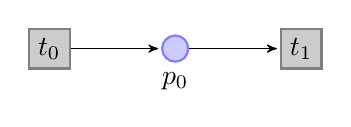
\begin{tikzpicture}[node distance=16mm, >=stealth', bend angle=45, auto]
          \node[place] (p0) [label=below:$p_0$] {};
          
          \node [transition] (t0) [left of=p0] {$t_0$}
                edge [post] (p0);
          \node [transition] (t1) [right of=p0] {$t_1$}
                edge [pre] (p0);
        \end{tikzpicture}
      \caption{Un réseau de Petri très simple}
      \label{fig:simple_net}
    \end{figure}

    \begin{figure}[h]
      \centering
        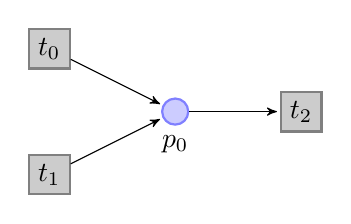
\begin{tikzpicture}[node distance=16mm, >=stealth', bend angle=45, auto]
          \node[place] (p0) [label=below:$p_0$] {};
          
          \node [transition] (t0) [left of=p0, yshift=8mm] {$t_0$}
                edge [post] (p0);
          \node [transition] (t1)[below of=t0] {$t_1$}
                edge [post] (p0);
          \node [transition] (t2) [right of=p0] {$t_2$}
                edge [pre] (p0);
        \end{tikzpicture}
      \caption{Un autre réseau de Petri très simple}
      \label{fig:simple_net2}
    \end{figure}

\end{document}
